
\begin{frame}{What do we do with different types of eigenvalues?}
	    Each interesting “case” of eigenvalues (real, imaginary, and repeated) is complementary to a case of resonance in 2d ODEs, so let’s discuss them together:
        
        \begin{center}
            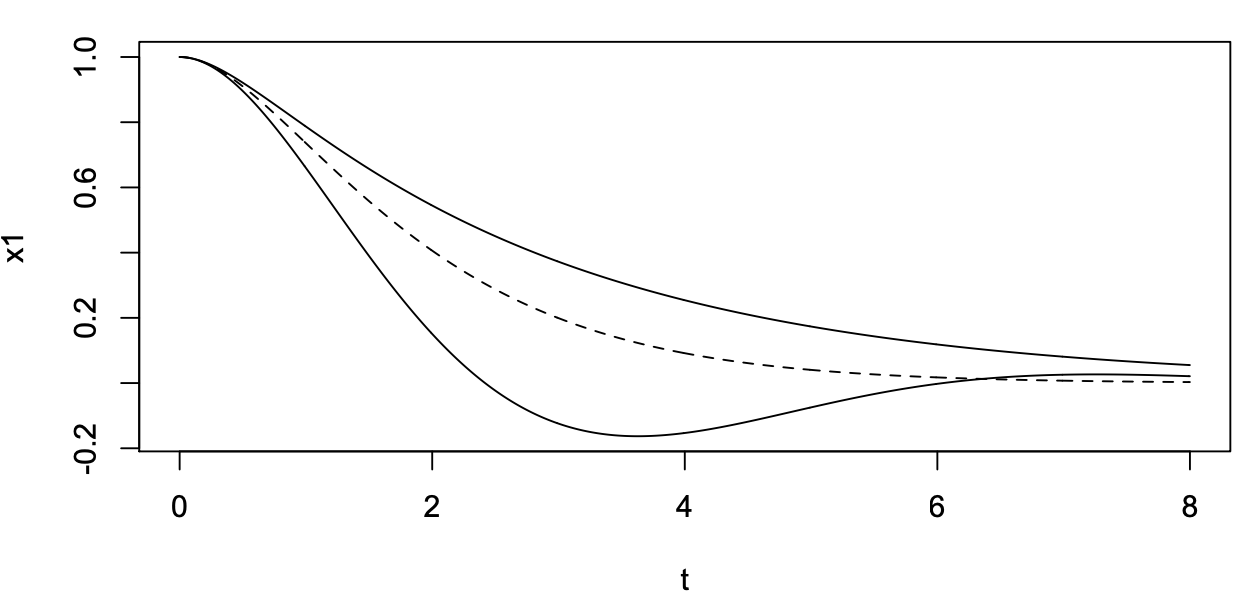
\includegraphics[width=0.5\textwidth]{./images/eigenvalue-types-1.png}
        \end{center}
	\end{frame}
	
	\begin{frame}{Overdamping: two real eigenvalues}
	    \begin{itemize}
	        \item When a system has two real eigenvalues, it will have two real eigenvectors, so the solution will be a combination of exponentials in the form 
            
            $$ae^{\lambda_1t} + be^{\lambda_2t}$$
            
            \item For negative lambdas, this produces exponential decay.
            
            \item
            \begin{columns}[onlytextwidth,T]
            \column{\dimexpr\linewidth-40mm-5mm}
        	    At large t, greater eigenvalue dominates behavior, so how fast the system approaches to 0 is determined by the larger eigenvalue.
        	
        	\column{40mm}
        	    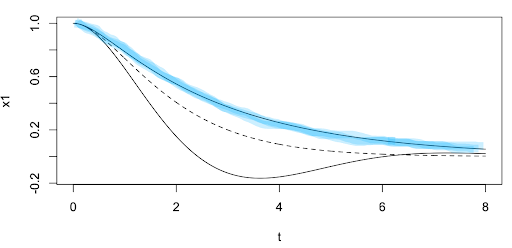
\includegraphics[width=40mm]{./images/eigenvalue-types-3.png}
    	    \end{columns}
	    \end{itemize}
	\end{frame}
	
	\begin{frame}{Underdamping: imaginary or complex eigenvalues}
	    \begin{itemize}
	        \item You can still solve the system of differential equations as usual, but your solutions will be complex:
            
            $$(a_1j + b_1)e^{c_1j + d_1} + (a_2j + b_2)e^{c_2j + d_2}$$
            
            \item You can rearrange terms and apply Euler’s formula to write each term as a real exponential multiplied by a sinusoid
            $$e^{d_1}(\alpha_1sin(...) + \beta_1cos(...)) + e^{d_2}(\alpha_2sin(...) + \beta_2cos(...))$$
            
            \item
            \begin{columns}[onlytextwidth,T]
            \column{\dimexpr\linewidth-40mm-5mm}
        	    If $d_1$ and $d_2$ are negative, then you can think of this as a sinusoid where the amplitude decays to 0
        	
        	\column{40mm}
        	    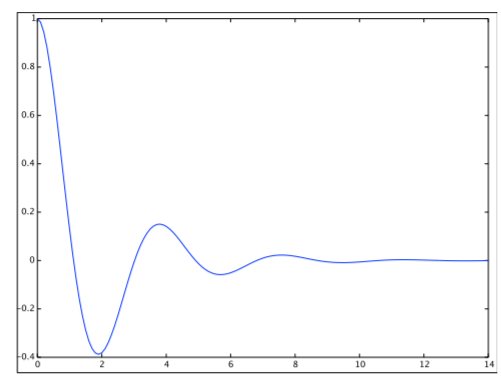
\includegraphics[width=40mm]{./images/eigenvalue-types-2.png}
    	    \end{columns}
	    \end{itemize}
	\end{frame}
	
	\begin{frame}{Critical Damping: repeated eigenvalue}
	    \begin{itemize}
	        \item You only get one linearly independent eigenvector. 
            
            \item So, arbitrarily choose the second column of your $V$ matrix (making sure it is linearly independent from the eigenvector $v_1$)
            
            \item Compute $A_v$ using the change of basis diagram $A_v = V^{-1}AV$
            
            \item This gives you an upper-triangular matrix
            
            \item The bottom row of the matrix gives you an equation in one variable (only depends on the second component of $x_v$), which you can solve to get something in the form of $x_{v,2} = ae^{\lambda{t}}$
	    \end{itemize}
	\end{frame}
	
	\begin{frame}{Critical Damping: repeated eigenvalue}
	    \begin{itemize}
	        \item The top row of the matrix depends on both components of $x_v$, but you can plug in the value you got for $x_{v,2}$ and then solve for $x_{v,1}$
            
            \item If you solve this differential equation (which is a diff eq with a non-constant input*), you’ll get an equation in the form:
            
            $$x(t) = c_1e^{-\lambda{t}} + c_2te^{-\lambda{t}}$$
            
            \item
            \begin{columns}[onlytextwidth,T]
            \column{\dimexpr\linewidth-40mm-5mm}
        	    \textbf{The critically damped case gives us the fastest-decaying exponential that doesn’t oscillate}
        	
        	\column{40mm}
        	    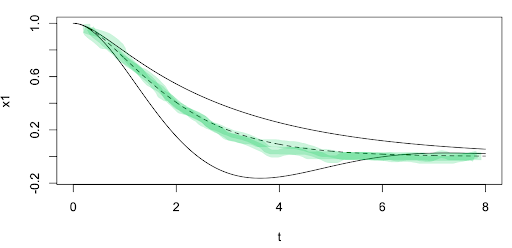
\includegraphics[width=40mm]{./images/eigenvalue-types-4.png}
    	    \end{columns}
	    \end{itemize}
	    
	    *You can solve this using the formula $x_p(t) = x_0e^{\lambda{t}} + \int_0^t u(\tau)e^{\lambda(t-\tau)} d\tau$
	\end{frame}
	

